\documentclass[final,5p,times,twocolumn,authoryear]{elsarticle}
\usepackage{amssymb}
\usepackage{lipsum}

\newcommand{\kms}{km\,s$^{-1}$}
\newcommand{\msun}{$M_\odot}

\journal{Machine Learning Research}


\begin{document}

\begin{frontmatter}

%% Title, authors and addresses

%% use the tnoteref command within \title for footnotes;
%% use the tnotetext command for theassociated footnote;
%% use the fnref command within \author or \affiliation for footnotes;
%% use the fntext command for theassociated footnote;
%% use the corref command within \author for corresponding author footnotes;
%% use the cortext command for theassociated footnote;
%% use the ead command for the email address,
%% and the form \ead[url] for the home page:
%% \title{Title\tnoteref{label1}}
%% \tnotetext[label1]{}
%% \author{Name\corref{cor1}\fnref{label2}}
%% \ead{email address}
%% \ead[url]{home page}
%% \fntext[label2]{}
%% \cortext[cor1]{}
%% \fntext[label3]{}

\title{Less Is More: Linear Layers on CLIP Features as Powerful VizWiz Model}

%% use optional labels to link authors explicitly to addresses:
%% \author[label1,label2]{}
%% \affiliation[label1]{organization={},
%%             addressline={},
%%             city={},
%%             postcode={},
%%             state={},
%%             country={}}
%%
%% \affiliation[label2]{organization={},
%%             addressline={},
%%             city={},
%%             postcode={},
%%             state={},
%%             country={}}

\author[first, second, third]{Yousef Kotp, Adham Mohammed, Mohammed Farid}
\affiliation[first]{organization={@Alexandria University},%Department and Organization
            addressline={yousefkotp@outlook.com},
            city={Alexandria},
            country={Egypt}}
            
\affiliation[second]{organization={@Alexandria University},%Department and Organization
            city={Alexandria},
            country={Egypt}}
            
\affiliation[third]{organization={@Alexandria University},%Department and Organization
            city={Alexandria},
            country={Egypt}}


%% Abstract
\begin{abstract}

In our groundbreaking research, we have developed a cutting-edge model that will revolutionize visual question answering (VQA) tasks. By leveraging the power of OpenAI's CLIP model, which possesses the remarkable ability to understand both images and text, we have created a lightweight solution that surpasses its counterparts. Our model has \textbf{achieved an impressive 54\% success rate and \textbf{ranked 4th in the official leaderboard} for the challenge in Task 1: Predict Answer to a Visual Question}, establishing itself as one of the top performers. However, we didn't stop there. We confronted the challenge of complexity head-on, devising a method to simplify the current VQA architectures. Our secret weapon includes curating answer vocabulary and incorporating an auxiliary loss for the answer type, which has unlocked the true potential of our model. This technique not only improved our training process but also paved the way for even more remarkable results. Additionally, by utilizing the mask obtained from this loss, we created a gate for the answers, resulting in a significant performance boost for our model. In Task 2: Predict Answerability of a Visual Question, our model achieved an astonishing \textbf{average precision of 73.15}\% and \textbf{ranked 3rd in the official leaderboard}. These tasks were part of the VizWiz Visual Question Answering Grand Challenge.

\end{abstract}


%%Graphical abstract
% \begin{graphicalabstract}
% \includegraphics{JHEAP_cover_image.pdf}
% \end{graphicalabstract}

%%Research highlights
% \begin{highlights}
% \item Research highlight 1
% \item Research highlight 2
% \end{highlights}



\begin{keyword}
%% keywords here, in the form: keyword \sep keyword, up to a maximum of 6 keywords
VizWiz \sep Visual Question Answering \sep Open AI's CLIP model\sep VQA
\end{keyword}


\end{frontmatter}

%\tableofcontents

%% main text

\section{Introduction}
\label{introduction}

In recent years, the field of visual question answering (VQA) has seen the development of numerous new architectures that have been applied to various datasets such as VQAv2, GQA, and VizWiz-VQA. The VizWiz dataset stands out from other VQA datasets due to the presence of several challenges in the data. For instance, questions in this dataset may be unanswerable due to missing information in the accompanying images, or the image quality itself may be exceptionally poor. Additionally, the questions in the dataset are not formulated based on rigid rules but rather tend to be colloquial and informal in nature.

In the previous year, the winning team in the VizWiz-VQA challenge employed an extension of OSCAR, a popular VQA model. They enhanced their model by incorporating an optical character recognition (OCR) module and introducing reference image matching. Their final system consisted of an ensemble of 96 individual models. Ensembles are crucial for achieving competitive results in VQA, but they come with a significant cost in terms of training.

It is worth noting that while many new architectures have emerged in recent years, the development and training of VQA models can be computationally expensive and resource-intensive. The complexity of the models, the size of the datasets, and the need for extensive training to optimize performance all contribute to the high cost associated with these approaches. Nonetheless, the continuous advancement of VQA architectures and techniques holds great promise for tackling the challenges posed by diverse and challenging datasets like VizWiz.

\begin{figure}
	\centering 
	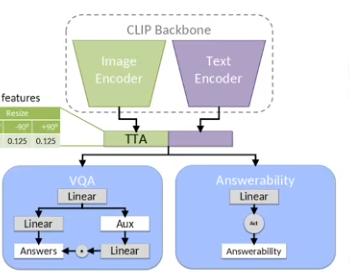
\includegraphics[width=0.4\textwidth]{model_architecture.png}	
	\caption{Our Proposed Model Architecture} 
	\label{fig_mom0}%
\end{figure}

Our approach places emphasis on simplicity and usability in the context of visual question answering (VQA). We adopt a strategy that involves utilizing pre-trained image and text encoders from CLIP and focusing solely on training a straightforward classification head. The CLIP model itself is built upon convolutional neural networks (CNN) for image encoding and Vision Transformer for text encoding. It leverages the power of a Transformer for text representation.

To facilitate the alignment of images and text, the CLIP model is pre-trained on a vast dataset of 400 million image-text pairs. This pre-training phase employs a contrastive objective, enabling both image and text modalities to be embedded within the same space. This integration ensures that images and corresponding text descriptions can be effectively compared and matched. Furthermore, due to the large-scale training of CLIP, the model also possesses optical character recognition (OCR) capabilities, enhancing its ability to extract and understand text from images.



%%%%%%%%%%%%%%%%%%%%%%%%%% RELATED WORK %%%%%%%%%%%%%%%%%%%%%%%
% \section{Related Work}



%%%%%%%%%%%%%%%%%%%%%%%%%% PROPOSED METHOD %%%%%%%%%%%%%%%%%%%%%%%
\section{Proposed Method}
\subsection{Building the Perfect Vocab}

We curated the perfect vocabulary for a Visual Question Answering (VQA) model using the VizWiz dataset. The goal is to select the most representative and common answers for each question in the dataset.

The function follows a specific policy to build the answer vocabulary. For each question in the dataset, there are multiple answers available (typically 10).

Next, for each question in the dataset, the function counts the frequency of each answer using an intermediate counter. This counter keeps track of how many times each answer occurs for a particular question.

Once the answers for a question are counted, the function checks for any ties in the answer frequencies. If there is only one most frequent answer, it is selected as the answer for that question, and it is assigned to the corresponding row in the dataframe.

However, if there is a tie in the answer frequencies, the function looks at the most common answer in the entire dataset. This step ensures that if multiple answers are equally common across different questions, the most common answer overall is chosen. Again, if there is a clear winner, it is assigned to the corresponding row in the dataframe.

In the case where there is still a tie after considering the overall most common answer, the function utilizes pairwise Levenshtein distance. It calculates the Levenshtein distance between all the tied answers and selects the answer that has the minimum total distance from all the other tied answers. This answer is considered the most representative answer for the tied group.

Finally, after iterating through all the questions in the dataset, the function returns the curated answer vocabulary, stored in the dataframe.

By following this policy, the function ensures that the curated vocabulary consists of the most frequent and representative answers for each question in the VizWiz dataset, providing a reliable basis for training a visual question answering model. The number of distinct answer (classes) becomes 5410.

\subsection{Auxilary Loss}

We used an auxiliary loss called the "Answer Type Gate" to improve the VQA model. This loss is designed to learn an answer masking mechanism based on the answer types, which helps the model better understand and handle different types of answers. The answer types considered in this approach include "numbers," "yes/no," "others," and "unanswerable,"

To train the auxiliary loss, the answer types are determined by performing regular expression matching on the best-selected answer for each image-question pair in the dataset. This means that for every question, the most suitable answer type is identified based on its content.

The predictions for answer types are learned using a linear projection, which maps the answer type predictions to a vector of the same dimension as the number of possible answer classes. In this case, the dimension is 5410, representing the vocabulary size of the answers.

After the linear projection, a sigmoid layer is applied to obtain probabilities for each answer type. These probabilities are then multiplied element-wise with the logits (scores) of the answer vocabulary. This multiplication effectively masks answers that do not correspond to the current answer type during inference. By applying this masking mechanism, the model can focus on generating answers that are relevant to the detected answer type.

Both the intermediate answer type prediction and the final answer classification contribute to the loss function. The two cross-entropy losses, one for the intermediate answer type prediction and the other for the final answer classification, are weighted equally in the overall loss calculation. This means that both tasks are considered equally important during training, encouraging the model to effectively predict both the answer type and the answer itself.

\begin{figure}
	\centering 
	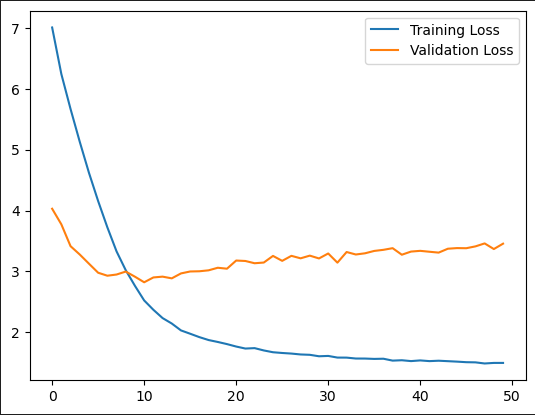
\includegraphics[width=0.4\textwidth]{training_losses.png}	
	\caption{Training and Validation Losses} 
	\label{fig_mom0}%
\end{figure}

By incorporating the Answer Type Gate auxiliary loss, the VQA model gains the ability to understand and distinguish different types of answers. This mechanism helps the model generate more accurate and contextually appropriate answers by masking irrelevant options during inference, improving its overall performance on the VQA task.


%%%%%%%%%%%%%%%%%%%%%%%%%% SETUP %%%%%%%%%%%%%%%%%%%%%%%
\section{Experimental Setup}


The model was trained for a total of 50 epoch, we took the best performing model which turned out to be at epoch number 45, the training was done primarily on Kaggle using P100 accelerator. We usd a learning rate of 5e-4 with a batch size of 32 (64 was bad in terms of variance). However, we used 0.05 of the training data as test date, we didn't use the official test dataset which affected the training very much. The experiment would give even better results if we didn't split it.



%%%%%%%%%%%%%%%%%%%%%%%%%% EVALUATION %%%%%%%%%%%%%%%%%%%%%%%
\section{Evaluation}
\subsection{Evaluation Metrics}
Task 1: Predict Answer to a Visual Question
Given an image and question about it, the task is to predict an accurate answer. Inspired by the VQA challenge, we use the following accuracy evaluation metric which equals minimum of either one or the number of humans that provided that answer divided by three.Following the VQA challenge, we average over all 10 choose 9 sets of human annotators. The team which achieves the maximum average accuracy for all test visual questions wins this challenge.

Task 2: Predict Answerability of a Visual Question
Given an image and question about it, the task is to predict if the visual question cannot be answered (with a confidence score in that prediction). The confidence score provided by a prediction model is for ‘answerable’ and should be in [0,1]. We use Python’s average precision evaluation metric which computes the weighted mean of precisions under a precision-recall curve. The team that achieves the largest average precision score for all test visual questions wins this challenge.

\begin{figure}
	\centering 
	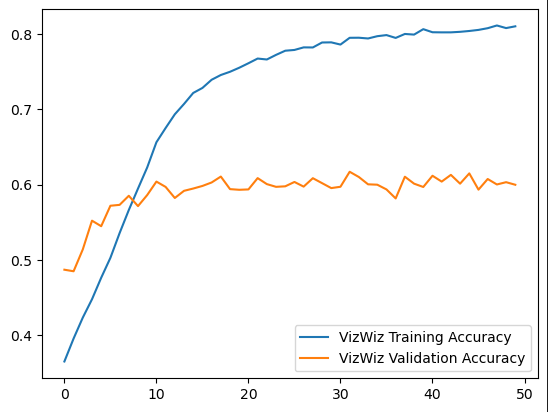
\includegraphics[width=0.4\textwidth]{training_vizwiz_accuracy.png}	
	\caption{Training and Validation VizWiz Accuracy} 
	\label{fig_mom0}%
\end{figure}

\subsection{Results}
he results table (Table 1) presents the performance of a VQA model on various metrics. The metrics include VizWiz accuracy, accuracy, and answerability.

For VizWiz accuracy, the model achieved a training accuracy of 80.4\% and a validation accuracy of 61.5\%. This metric indicates how well the model performs on the VizWiz dataset, which is a real-world image dataset containing challenging visual question answering scenarios.

The accuracy metric measures the overall correctness of the model's predictions. The training accuracy achieved by the model is 76.4\%, while the validation accuracy is 48.0\%. This metric provides insight into the model's ability to generate accurate answers across different question types and image contexts.

The answerability metric focuses on the model's capability to identify questions that are unanswerable. The training and validation answerability scores are 80.2\% and 79.8\%, respectively. This metric assesses the model's skill in determining when a question does not have a meaningful answer based on the given image.

Overall, the results indicate that the model performs relatively well in terms of VizWiz accuracy and answerability, achieving high scores in both training and validation phases. However, the accuracy metric suggests that there is room for improvement, as the model's performance is comparatively lower, especially on the validation set. These findings provide valuable insights for further optimizing the VQA model and enhancing its overall performance.






\section{Conclusion}

Our approach focuses on lightweight training by keeping the pre-trained CLIP backbone frozen, while still maintaining good accuracy. The OCR capabilities of CLIP, the large amount of pre-training data, and the multi-modality make CLIP an excellent feature extractor for this task. Unlike previous publications, the text Transformer is also used from CLIP. Although it was trained on alt-texts, it could be shown that meaningful representations of the questions are extracted without any fine-tuning. On the VizWiz VQA task we reach 61.5\% with a single model using ViT backbone on the validation dataset and 54\% on the test dataset.
\begin{table}
\begin{tabular}{l c c c} 
 \hline
 Metric & Training & Validation & \\
 \hline
 VizWiz Accuracy\, & 	80.4\, & 61.5 \\
 Accuracy\, & 76.4\, & 48.0 \\
 Answerability\, & 80.2\, & 79.8 \\
 \hline
\end{tabular}

\caption{Results table for different metrcis}

\label{Table1}
\end{table}


\appendix

\section{GitHub Code}
\label{this is amazing}
https://github.com/yousefkotp/Visual-Question-Answering/tree/main


\bibliographystyle{elsarticle-harv} 

%% else use the following coding to input the bibitems directly in the
%% TeX file.

\begin{thebibliography}{00}

% \bibitem[Author(year)]{label}
\bibitem[Danna Gurari, Qing Li, Abigale J. Stangl, Anhong Guo, Chi Lin, Kristen Grauman, Jiebo Luo, Jeffrey P. Bigham]{VizWiz} VizWiz Grand Challenge: Answering Visual Questions from Blind People (2018)


\end{thebibliography}

\end{document}

\endinput